% Created 2020-10-26 Mon 16:22
% Intended LaTeX compiler: pdflatex
\documentclass[presentation, aspectratio=169]{beamer}
\usepackage[utf8]{inputenc}
\usepackage[T1]{fontenc}
\usepackage{graphicx}
\usepackage{grffile}
\usepackage{longtable}
\usepackage{wrapfig}
\usepackage{rotating}
\usepackage[normalem]{ulem}
\usepackage{amsmath}
\usepackage{textcomp}
\usepackage{amssymb}
\usepackage{capt-of}
\usepackage{hyperref}
\RequirePackage{fancyvrb}
\usepackage[margin=0.5in]{geometry}
\usepackage[backend=bibtex]{biblatex}
\addbibresource{./../biblio.bib}
\author[A. Caliò]{Antonio Caliò\inst{1}}
\usetheme{default}
\date{}
\title{Introduction to SBT}
\institute{\inst{1}DIMES Dept., University of Calabria\\ Rende (CS), IT \\ a.calio@unical.it\\ Big Data Analytics - Computer Engineering for the IoT}
\titlegraphic{\begin{picture}(0,0) \put(200,200){\makebox(0,0)[rt]{
\includegraphics[width=3cm]{./img/logo_dimes.jpg}}} \end{picture}}}
\AtBeginSection[]{\begin{frame}<beamer>\frametitle{Presentation agenda}\tableofcontents[currentsection]\end{frame}}
\hypersetup{
 pdfauthor={},
 pdftitle={Introduction to SBT},
 pdfkeywords={},
 pdfsubject={},
 pdfcreator={Emacs 27.1 (Org mode 9.3)}, 
 pdflang={English}}
\begin{document}

\maketitle
\begin{frame}{Outline}
\tableofcontents
\end{frame}


\section{Introduction}
\label{sec:org5903384}
\begin{frame}[label={sec:orgd967ee4}]{Why?}
\begin{block}{Why a Build System?}
\begin{itemize}
\item As your project grows in complexity, compiling your source code "by hand" will soon become a nightmare!
For this reason you need a smart system to build your entire project.
\end{itemize}
\end{block}

\begin{block}{Why SBT?}
\begin{itemize}
\item It is  specifically built for java and scala projects. It represents the build tool of choice
for more  than 90\% of all Scala projects
\item It is typesafe and parallel
\item The compilation process is incremental
\item You can easily declare \emph{watches} over source file, so that they are compiled as  soon as SBT detects a change in the code
\item It can be extended with a number of community-driven plugins
\end{itemize}
\end{block}
\end{frame}


\section{Getting Started}
\label{sec:orgf6d871b}

\begin{frame}[label={sec:org4a564e3},fragile]{sbt by example}
 \begin{itemize}
\item First you need to download and install SBT following  \href{https://www.scala-sbt.org/1.x/docs/index.html}{\alert{this}} link
\item Create the root directory for your project 
\begin{verbatim}
mkdir proot
cd proot # move inside the folder
touch build.sbt # create the build file
\end{verbatim}
\item One way of building the project is by opening an interactive folder inside the project main folder
\begin{verbatim}
sbt
sbt:proot> compile
\end{verbatim}
The above command will build your project accordingly to what it is specified inside the file \texttt{build.sbt}
\end{itemize}
\begin{itemize}
\item You can create \emph{watches} over the files composing your project as follows:
\begin{verbatim}
sbt:proot> ~compile
\end{verbatim}
With the above instruction SBT will re-compile the project if anything change on disk
\end{itemize}
\end{frame}

\begin{frame}[label={sec:org3f67649},fragile]{Create a source file}
 \begin{columns}
\begin{column}{0.45\columnwidth}
\begin{itemize}
\item The tree structure of your SBT project must adhere to the following structure:

\begin{figure}[htbp]
\centering
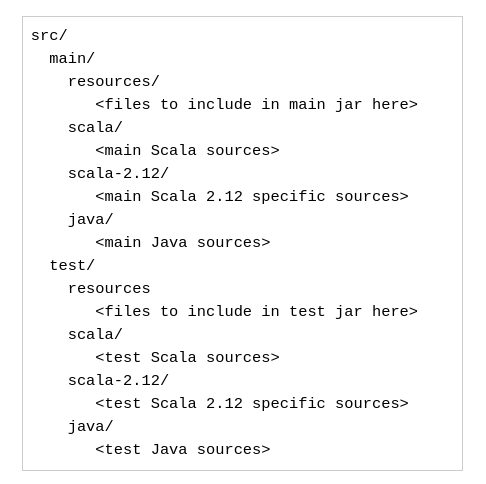
\includegraphics[width=3cm,height=4cm]{./img/dir-structure.png}
\caption{\label{fig:org7ba445d}sbt project dir structure}
\end{figure}
\end{itemize}
\end{column}

\begin{column}{0.45\columnwidth}
\begin{itemize}
\item All the scala source file goes into the src/main/scala subdirectory

\item Add the following class to that directory

\begin{verbatim}
package example

object Hello extends App {
  println("Hello")
}
\end{verbatim}
\end{itemize}
\end{column}
\end{columns}
\end{frame}


\begin{frame}[label={sec:org7ffa719},fragile]{Run your App}
 \begin{itemize}
\item first run \texttt{compile} once again
\item then issue the command \texttt{run} and you should be able to see the output of your program
\begin{figure}[htbp]
\centering
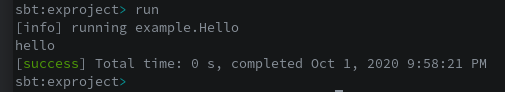
\includegraphics[width=150px]{./img/sbt-run.png}
\caption{\label{fig:org4d37e13}sbt run}
\end{figure}
\end{itemize}
\end{frame}

\begin{frame}[label={sec:org8529f28},fragile]{Setting the build.sbt file}
 \begin{itemize}
\item First, you assign a name to your project.
\item A good start for the build sbt file would be the following:
\end{itemize}
\tiny
\begin{verbatim}
ThisBuild / scalaVersion := "2.12.7"
ThisBuild / organization := "com.example"

lazy val hello = (project in file("."))
  .settings(
    name := "Hello"
  )
\end{verbatim}
\large
\begin{itemize}
\item Every time you update the sbt file you should call \texttt{reload} on the interactive shell in order
the updates to take effect

\begin{figure}[htbp]
\centering
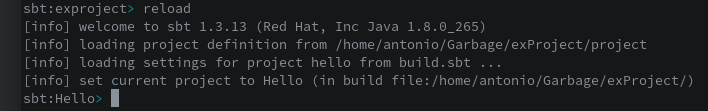
\includegraphics[width=200px,height=50px]{./img/sbt-reload.png}
\caption{\label{fig:orgd5af0c7}sbt reload}
\end{figure}
\end{itemize}
\end{frame}

\begin{frame}[label={sec:org434be15},fragile]{Enable testing}
 \begin{itemize}
\item Change the build.sbt as follows
\end{itemize}
\tiny
\begin{verbatim}
ThisBuild / scalaVersion := "2.12.7"
ThisBuild / organization := "com.example"

lazy val hello = (project in file("."))
  .settings(
    name := "Hello",
    libraryDependencies += "org.scalatest" %% "scalatest" % "3.0.5" % Test,
 )
\end{verbatim}
\large
\begin{itemize}
\item then for running the tests:
\end{itemize}
\tiny
\begin{verbatim}
sbt:Hello> reload
sbt:Hello> test
sbt:Hello> ~testQuick
\end{verbatim}
\end{frame}

\begin{frame}[label={sec:org71e909d},fragile]{Writing a test}
 \begin{itemize}
\item Under the \emph{src} folder create a test folder and save the following file:
\end{itemize}
\tiny
\begin{verbatim}
import org.scalatest._

class HelloSpec extends FunSuite with DiagrammedAssertions {
  test("Hello should start with H") {
    assert("hello".startsWith("H"))
  }
}
\end{verbatim}
\large
\begin{itemize}
\item Then you can reload the project an run the tests once again
\end{itemize}
\end{frame}
\begin{frame}[label={sec:orgba817a0},fragile]{Add a library dependency}
 \begin{itemize}
\item Dependencies are defined in the \texttt{build.sbt}  file.
\end{itemize}
\tiny
\begin{verbatim}
ThisBuild / scalaVersion := "2.12.7"
ThisBuild / organization := "com.example"

lazy val hello = (project in file("."))
  .settings(
    name := "Hello",
    libraryDependencies += "com.typesafe.play" %% "play-json" % "2.6.9",
    libraryDependencies += "com.eed3si9n" %% "gigahorse-okhttp" % "0.3.1",
    libraryDependencies += "org.scalatest" %% "scalatest" % "3.0.5" % Test,
  )
\end{verbatim}
\end{frame}

\begin{frame}[label={sec:orgdd9f51d},fragile]{Make a subproject}
 \begin{itemize}
\item You can include subproject inside your main one.
\end{itemize}
\tiny
\begin{verbatim}
ThisBuild / scalaVersion := "2.12.7"
ThisBuild / organization := "com.example"

lazy val hello = (project in file("."))
  .settings(
    name := "Hello",
    libraryDependencies += "com.eed3si9n" %% "gigahorse-okhttp" % "0.3.1",
    libraryDependencies += "org.scalatest" %% "scalatest" % "3.0.5" % Test,
  )

lazy val helloCore = (project in file("core"))
  .settings(
    name := "Hello Core",
  )

\end{verbatim}
\end{frame}

\begin{frame}[label={sec:org7c74aa8},fragile]{Add ScalaTest to the subproject}
 \begin{itemize}
\item Change the build.sbt as follows:
\end{itemize}
\tiny
\begin{verbatim}
ThisBuild / scalaVersion := "2.12.7"
ThisBuild / organization := "com.example"

val scalaTest = "org.scalatest" %% "scalatest" % "3.0.5"

lazy val hello = (project in file("."))
  .settings(
    name := "Hello",
    libraryDependencies += "com.eed3si9n" %% "gigahorse-okhttp" % "0.3.1",
    libraryDependencies += scalaTest % Test,
  )

lazy val helloCore = (project in file("core"))
  .settings(
    name := "Hello Core",
    libraryDependencies += scalaTest % Test,
  )
\end{verbatim}
\end{frame}

\begin{frame}[label={sec:org1c41e4e},fragile]{Broadcast Commands}
 \begin{itemize}
\item If you want any command sent to \texttt{hello} to be broadcaster to the \texttt{hellocore} project you can use the 
\texttt{aggregate} function.
\end{itemize}
\tiny
\begin{verbatim}
ThisBuild / scalaVersion := "2.12.7"
ThisBuild / organization := "com.example"

val scalaTest = "org.scalatest" %% "scalatest" % "3.0.5"

lazy val hello = (project in file("."))
  .aggregate(helloCore)
  .settings(
    name := "Hello",
    libraryDependencies += "com.eed3si9n" %% "gigahorse-okhttp" % "0.3.1",
    libraryDependencies += scalaTest % Test,
  )

lazy val helloCore = (project in file("core"))
  .settings(
    name := "Hello Core",
    libraryDependencies += scalaTest % Test,
  )
\end{verbatim}
\end{frame}

\begin{frame}[label={sec:org63f3c96},fragile]{Define dependencies}
 \begin{itemize}
\item if you want to define a dependency for a project you must use the \texttt{.dependsOn} function as follows:
\end{itemize}
\tiny
\begin{verbatim}
ThisBuild / scalaVersion := "2.12.7"
ThisBuild / organization := "com.example"

val scalaTest = "org.scalatest" %% "scalatest" % "3.0.5"

lazy val hello = (project in file("."))
  .aggregate(helloCore)
  .dependsOn(helloCore)
  .settings(
    name := "Hello",
    libraryDependencies += scalaTest % Test,
  )

lazy val helloCore = (project in file("core"))
  .settings(
    name := "Hello Core",
    libraryDependencies += "com.eed3si9n" %% "gigahorse-okhttp" % "0.3.1",
    libraryDependencies += scalaTest % Test,
  )
\end{verbatim}
\end{frame}

\begin{frame}[label={sec:org57a4a6d},fragile]{Add the Play-Json dependency}
 \tiny
\begin{verbatim}
ThisBuild / scalaVersion := "2.12.7"
ThisBuild / organization := "com.example"

val scalaTest = "org.scalatest" %% "scalatest" % "3.0.5"
val gigahorse = "com.eed3si9n" %% "gigahorse-okhttp" % "0.3.1"
val playJson  = "com.typesafe.play" %% "play-json" % "2.6.9"

lazy val hello = (project in file("."))
  .aggregate(helloCore)
  .dependsOn(helloCore)
  .settings(
    name := "Hello",
    libraryDependencies += scalaTest % Test,
  )

lazy val helloCore = (project in file("core"))
  .settings(
    name := "Hello Core",
    libraryDependencies ++= Seq(gigahorse, playJson),
    libraryDependencies += scalaTest % Test,
  )

\end{verbatim}
\end{frame}

\begin{frame}[label={sec:org3d7a9fe},fragile]{Add another source file}
 \begin{itemize}
\item Add a new source file under the folder \emph{core/src/main/scala/example}, name it \texttt{Wheater.scala}
\end{itemize}
\tiny
\begin{verbatim}
package example.core

import gigahorse._, support.okhttp.Gigahorse
import scala.concurrent._, duration._
import play.api.libs.json._

object Weather {
  lazy val http = Gigahorse.http(Gigahorse.config)

  def weather: Future[String] = {
    val baseUrl = "https://www.metaweather.com/api/location"
    val locUrl = baseUrl + "/search/"
    val weatherUrl = baseUrl + "/%s/"
    val rLoc = Gigahorse.url(locUrl).get.
      addQueryString("query" -> "New York")
    import ExecutionContext.Implicits.global
    for {
      loc <- http.run(rLoc, parse)
      woeid = (loc \ 0  \ "woeid").get
      rWeather = Gigahorse.url(weatherUrl format woeid).get
      weather <- http.run(rWeather, parse)
    } yield (weather \\ "weather_state_name")(0).as[String].toLowerCase
  }

  private def parse = Gigahorse.asString andThen Json.parse
}
\end{verbatim}
\end{frame}

\begin{frame}[label={sec:orgb9f5ceb},fragile]{Update the main class}
 \begin{itemize}
\item Create the file \texttt{Hello.scala} under \texttt{src/main/scala/example/Hello.scala}, then run the app.
\end{itemize}
\tiny
\begin{verbatim}
package example

import scala.concurrent._, duration._
import core.Weather

object Hello extends App {
  val w = Await.result(Weather.weather, 10.seconds)
  println(s"Hello! The weather in New York is $w.")
  Weather.http.close()
}
\end{verbatim}
\end{frame}

\begin{frame}[label={sec:org617d990},fragile]{Add a plugin}
 \begin{itemize}
\item To add a plugin you must add a file \texttt{plugins.sbt} under the \texttt{project} folder.
Here we add the \texttt{sbt-native-packager} plugin. It is very useful as it
\end{itemize}
\begin{verbatim}
addSbtPlugin("com.typesafe.sbt" % "sbt-native-packager" % "1.3.4")
\end{verbatim}
\end{frame}

\begin{frame}[label={sec:orga1860b4},fragile]{Enable a plugin}
 \begin{itemize}
\item Change the \texttt{build.sbt} file as follows
\end{itemize}
\begin{verbatim}
ThisBuild / scalaVersion := "2.12.7"
ThisBuild / organization := "com.example"

val scalaTest = "org.scalatest" %% "scalatest" % "3.0.5"
val gigahorse = "com.eed3si9n" %% "gigahorse-okhttp" % "0.3.1"
val playJson  = "com.typesafe.play" %% "play-json" % "2.6.9"

lazy val hello = (project in file("."))
  .aggregate(helloCore)
  .dependsOn(helloCore)
  .enablePlugins(JavaAppPackaging)
  .settings(
    name := "Hello",
    libraryDependencies += scalaTest % Test,
  )

lazy val helloCore = (project in file("core"))
  .settings(
    name := "Hello Core",
    libraryDependencies ++= Seq(gigahorse, playJson),
    libraryDependencies += scalaTest % Test,
  )
\end{verbatim}
\end{frame}

\begin{frame}[label={sec:org091dc72}]{Distribute your project}
\begin{itemize}
\item once you enabled the packager plugin, you can create:
\begin{enumerate}
\item a .zip distribution. You just need to run: \alert{dist} inside the console
\item a docker image. You just need to tun \alert{Docker/publishLocal} inside the console
\end{enumerate}
\end{itemize}
\end{frame}


\section{Build Structure}
\label{sec:orga8ced04}

\begin{frame}[label={sec:org14d636e},fragile]{Create a new project}
 \begin{itemize}
\item You can create a new project with the \texttt{sbt new} command 
(you need at least the version 0.13.13 of sbt).
\begin{figure}[htbp]
\centering
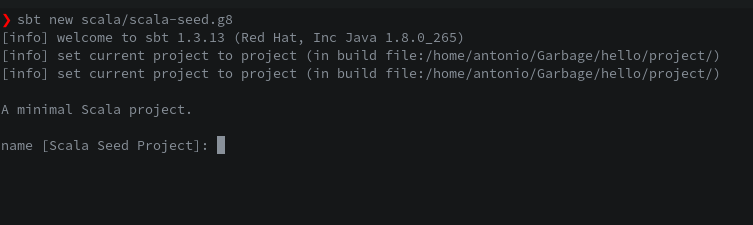
\includegraphics[width=.9\linewidth]{./img/sbt-new.png}
\caption{\label{fig:org569ce6a}Sbt-new}
\end{figure}

\item \texttt{socala/scala-seed.g8} is a template that will initialize the directory structure of you project.
There are several templates, but this is always a good starting point for most of the projects
\end{itemize}
\end{frame}

\begin{frame}[label={sec:orga4be23b}]{Understanding the directory structure}
\begin{columns}
\begin{column}{0.45\columnwidth}
\begin{itemize}
\item In sbt's terminology, the base directory is where the build.sbt is located.
This can be regarded as root folder of your project
\item Source Code directory. The source code structure resembles the one of Maven. 
Every path is relative to the source base directory
\end{itemize}
\end{column}

\begin{column}{0.45\columnwidth}
\begin{center}
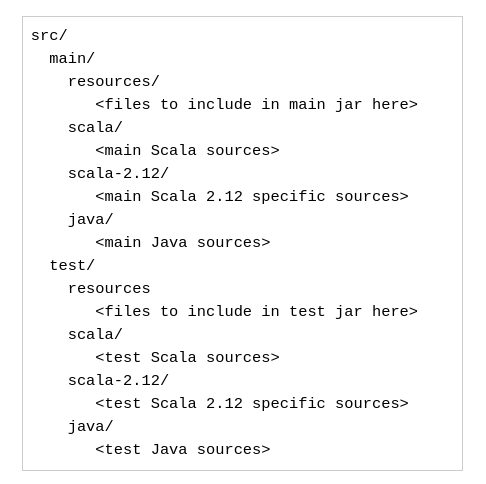
\includegraphics[width=.9\linewidth]{./img/dir-structure.png}
\end{center}
\end{column}
\end{columns}
\end{frame}


\begin{frame}[label={sec:org19edb89},fragile]{Build definition files}
 \begin{columns}
\begin{column}{0.45\columnwidth}
\begin{itemize}
\item The main file is the \texttt{build.sbt}
\item There are other support files located in other sub-directories of the base directory.
For instance we can have the \texttt{Dependencies.scala} under the project subdirectory.
\item Under the project directory you can also have a \texttt{plugins.sbt} file where you define the 
plugin involved in the process of building your project
\end{itemize}
\end{column}
\begin{column}{0.5\columnwidth}
\begin{figure}[htbp]
\centering
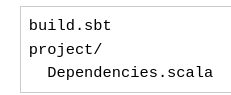
\includegraphics[width=.9\linewidth]{./img/dep-file.png}
\caption{\label{fig:org6d288fd}Dependencies file}
\end{figure}
\end{column}
\end{columns}
\end{frame}


\section{Build Definition}
\label{sec:org55064d1}

\begin{frame}[label={sec:org7bebb42},fragile]{What is a build definition?}
 A build definition is defined in the \texttt{build.sbt} file and it consists of a collection of subprojects.
A subproject is declared as follows:
\tiny
\begin{verbatim}
lazy val root = (project in file("."))
  .settings(
    name := "Hello",
    scalaVersion := "2.12.7"
  )
\end{verbatim}
\large   
   A subproject is represented by a series of key/value pairs, listed under the \texttt{.settings()} method.
\end{frame}

\begin{frame}[label={sec:org7a7a94f}]{How to defines settings}
\begin{itemize}
\item a key-value pair is called \emph{setting expression}. A \emph{setting expression} has the following structure:
\begin{figure}[htbp]
\centering
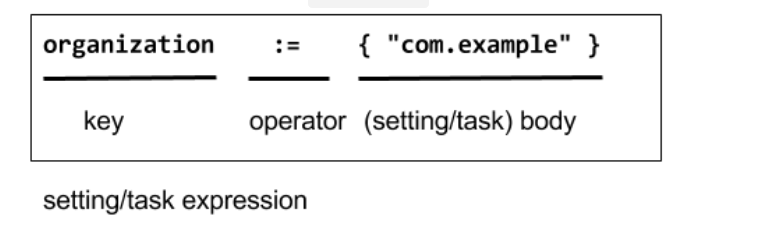
\includegraphics[width=100px]{./img/setting-expression.png}
\caption{\label{fig:org02a0ebb}Setting Expression}
\end{figure}

\item There are three parts:
\begin{enumerate}
\item Left-hand side: \alert{key}
\item \alert{Operator}
\item Right-hand side: \alert{body}
\end{enumerate}
\end{itemize}
\end{frame}

\section{Library Dependencies}
\label{sec:orgb6551c8}
\begin{frame}[label={sec:org67d1b05},fragile]{Adding library dependencies}
 \begin{itemize}
\item To depend on third-party libraries there are two options.
\begin{enumerate}
\item Drop the jars into \texttt{lib/} folder -- so you would have an \emph{unmanaged} dependency
\item Express the dependency in the \texttt{build.sbt} file -- so you would have a \emph{managed} dependency
\end{enumerate}
\end{itemize}
\begin{verbatim}

val derby = "org.apache.derby" % "derby" % "10.4.1.3"

ThisBuild / organization := "com.example"
ThisBuild / scalaVersion := "2.12.10"
ThisBuild / version      := "0.1.0-SNAPSHOT"

lazy val root = (project in file("."))
  .settings(
    name := "Hello",
    libraryDependencies += derby
  )

\end{verbatim}
\end{frame}

\begin{frame}[label={sec:org643938d},fragile]{Types of dependency}
 There are two type of dependencies:
\begin{itemize}
\item \emph{unmanaged} - if you just drop a jar file inside the \texttt{lib} folder
\item \emph{managed} - if you download the dependency from a respository
\end{itemize}
\end{frame}
\begin{frame}[label={sec:org21dbeff},fragile]{Unmmanaged dependency}
 \begin{itemize}
\item Unmanaged dependencies work like this: add jars to lib and they will be placed on the project classpath
\item Dependencies in lib go on all the classpaths (for compile, test, run, and console). 
If you wanted to change the classpath for just one of those, 
you would adjust Compile / dependencyClasspath or Runtime / dependencyClasspath for example.
\item You do not need to change anything in the \texttt{build.sbt} file in order to use unmanaged dependencies,
unless you want to override some configuration, for instance changing the base directory for the 
unmanaged dependencies:
\begin{verbatim}
unmanagedBased := baseDirectory.value / "custom_lib_direcotry"
\end{verbatim}
\end{itemize}
\end{frame}

\begin{frame}[label={sec:orgb2f9c11},fragile]{Managed dependency}
 \begin{itemize}
\item You define a managed dependency via the \texttt{libraryDependencies} key
\item A new dependency looks like this:
\end{itemize}
\tiny
\begin{verbatim}
libraryDependencies += groupId % artifactId % revision [% configurataion]
\end{verbatim}
\large
\begin{itemize}
\item You can also define a sequence of dependencies and add them with the ++= operator, like this:
\end{itemize}
\tiny
\begin{verbatim}
libraryDependencies ++= Seq(
  groupID % artifactID % revision,
  groupID % otherID % otherRevision
)
\end{verbatim}
\end{frame}

\begin{frame}[label={sec:org706b15e},fragile]{Getting the right Scala version with \%\%}
 \begin{itemize}
\item When you use the definition: "organization \%\% moduleName \% version" as opposed to "organization \% moduleName \% version",
sbt will add the Scala version to the artifact name.
\item Therefore the following definition:
\end{itemize}
\tiny
\begin{verbatim}
libraryDependencies += "org.scala-tools" % "scala-stm_2.11" % "0.3"
\end{verbatim}
\large
is equivalent to:
\tiny
\begin{verbatim}
libraryDependencies += "org.scala-tools" %% "scala-stm" % "0.3"
\end{verbatim}
\large
\begin{itemize}
\item The \%\% operator is very useful as many Scala libraries are compiled for multiple Scala versions. 
In this way you can select the version that better fits your project
\end{itemize}
\end{frame}
\begin{frame}[label={sec:org85e6ac2},fragile]{Resolvers}
 \begin{itemize}
\item Not all the packages live on the same server. sbt uses Maven2 repository by default. But if your dependency is 
on another repository you need to add a \emph{resolver} inside your build.sbt file, so that Ivy can find the dependency.

\item To add a resolver, here is the syntax:
\end{itemize}
\tiny
\begin{verbatim}
// resolvers += name at location
resolvers += "Sonatype OSS Snapshots" at "https://oss.sonatype.org/content/repositories/snapshots"
// if you have a local maven repository
resolvers += "Local Maven Repository" at "file://"+Path.userHome.absolutePath+"/.m2/repository"
\end{verbatim}
\end{frame}
\end{document}